\documentclass[12pt]{article}
\usepackage[margin=1in]{geometry}
\usepackage{relsize}
\usepackage{amssymb}
\usepackage{amsmath}
\usepackage{enumitem}
\usepackage{tikz}
\usetikzlibrary{automata,positioning}

\hyphenpenalty=10000
\setlength{\parindent}{0pt}

\newcommand\bicond{\mathrel{\leftrightarrow}}
\newcommand\bufprob{\vspace{2.0in}}
\newcommand\bufsub{\vspace{1.0in}}
\let\union\cup
\let\intersect\cap

\newenvironment{answer}{\larger[2]}{}

\begin{document}

\begin{center}
CS 441: Discrete Structures for Computer Science \\
{\smaller[1] Spring 2020} \\

\vspace {0.25in}

Practice Worksheet for remaining sections
\end{center}

\vspace{0.25in}

{\smaller[1]
\textbf{Username (abc123):} \rule{1.25in}{0.4pt}
}

\begin{center}
    {\large Section 9.1}
\end{center}

\begin{enumerate} % start main problems

% PROBLEM 1 (9.1 #1 (d))

\item[1. (d)] List the ordered pairs in the relation $R$ from $A = \{ 0,1,2,3,4 \}$ to $B = \{ 0, 1, 2, 3 \}$, where $(a,b) \in R$ if and only if $a | b$. Recall that $a | b$ means that a divides b or that $b = n \times a$ for some $n \in \mathbb{Z}$ (the integers).
\bufprob
%


% PROBLEM 2 (9.1, #3 (b) (e))

\item[3.] For each of these relations on the set $\{ 1,2,3,4 \}$, decide whether it is reflexive, whether it is symmetric, whether it is antisymmetric, and whether it is transitive.

\begin{enumerate}
    \item[(b)] $\{ (1,1), (1,2), (2,1), (2,2), (3,3), (4,4) \}$.
    
    \item[(e)] $\{ (1,1), (2,2), (3,3), (4,4) \}$.
    
    
\end{enumerate}

\newpage


% PROBLEM 3 (9.1 #7 (a) (b))

\item[7.] Determine whether the relation R on the set of all integers is reflexive, symmetric, antisymmetric, and/or transitive, where $(x,y) \in R$ if and only if:
%
\begin{enumerate}

\item[(a)] $x \neq y$.

\item[(b)] $xy \geq 1$.

\end{enumerate}
%

\bufprob


% PROBLEM 4 (9.1 #35 (a) (c))

For the following problem, let:

\begin{align*}
    R_2 &= \{ (a,b) \in R^2 | a \geq b \}, \text{ the greater than or equal to relation} \\
    R_3 &= \{ (a, b) \in R^2 | a < b \}, \text{ the less than relation} \\
    R_4 &= \{ (a, b) \in R^2 | a \leq b \}, \text{ the less than or equal to relation} \\
    R_6 &= \{ (a, b) \in R^2 | a \neq b \}, \text{ the unequal to relation} \\
\end{align*}

\item[35.] Find the following relations:

\begin{enumerate}
    \item[(a)] $R_2 \cup R_4$.
    
    
    \item[(c)] $R_3 \cap R_6$.
    
    
\end{enumerate}

\newpage

\begin{center}
    {\large Sections 4.1 to 4.3}
\end{center}


% PROBLEM 5 (4.1 #13 (a) (b))

\item[13.]  What are the quotient and remainder when:

\begin{enumerate}
    \item[(a)] 19 is divided by 7?
    
    
    \item[(b)] -111 is divided by 11?
    
    
\end{enumerate}
\bufsub

% Problem 6 (4.1 #15 (c))

\item[15. (c)] What time does a 12-hour clock read 100 hours after it reads 6:00?
\bufsub 

% Problem 7 (4.1 #29 (a) (c))

\item[29.] Find a \emph{div} m and a \emph{mod} m when:

\begin{enumerate}
    \item[(a)] a = 228, m = 119.
    
    
    \item[(c)] a = -10101, m = 333.
    
    
\end{enumerate}
\bufsub

% Problem 8 (4.1 #35 (b) (c))

\item[35.] Decide whether each of these integers is congruent to 5 modulo 17.

\begin{enumerate}
    \item[(b)] 103
    
    
    \item[(c)] -29
    
    
\end{enumerate}
\newpage

%Problem 9 (4.2 #1 (a) (b))

\item[1.] Convert the decimal expansion of each the these integers to a binary expansion.

\begin{enumerate}
    \item[(a)] 231
    
    
    \item[(b)] 4532
    
    
\end{enumerate}
\bufsub

%Problem 10 (4.2 #6 (a))

\item[6. (a)] Convert the binary expansion of (1111 0111$)_{2}$ to an octal expansion.
\bufsub

%Problem 11 (4.2 #6 (c))

\item[6. (c)] Convert the binary expansion of (111 0111 0111 0111$)_2$ to a hexadecimal expansion.                               
\bufsub

%Problem 12 (4.3 #3 (a) (b))

\item[3.] Find the prime factorization of each of these integers.

\begin{enumerate}
    \item[(a)] 88
    
    
    \item[(b)] 126
    
    
\end{enumerate}
\bufsub

%Problem 13 (4.3 #15)

\item[15.] Which positive integers less than 30 are relatively prime to 30?
\newpage

%Problem 14 (4.3 #18)

\item[18.] We call a positive integer \emph{perfect} if it equals the sum of its positive divisors other than itself. Show that 496 is perfect.
\bufsub

%Problem 15 (4.3 #24)

\item[24.] Find gcd(100, 125) and lcm(100, 125) and verify that gcd(100, 125) $\times$ lcm(100, 125) = $100 \times 125$.
\bufsub

%Problem 16 (4.3 #33 (d))

\item[33.] Use the Euclidean Algorithm to find gcd(12345, 54321).

\newpage

\begin{center}
    {\large Section 10.1}
\end{center}

%Problem 17 (10.1 #3)

\item[3.] Determine whether the graph shown has directed or undirected edges, whether it has multiple edges, and whether it has one or more loops. Use your answers to determine the type of graph. (Refer to Table 1 on page 676 of the textbook).

\hspace{50.0mm}
%Use tikzpicture to make a visual representation of the graph
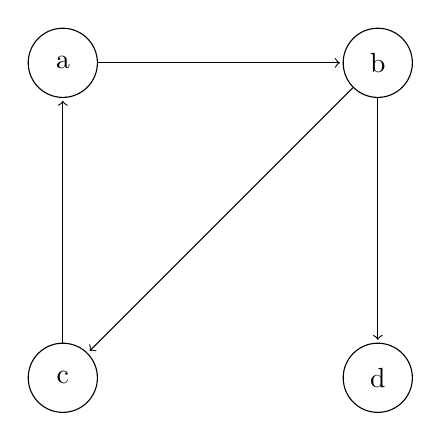
\begin{tikzpicture}[shorten >=1pt, node distance=4cm, on grid, auto]
    \node[state] (0) {a};
    \node[state] (1) [right=of 0] {b};
    \node[state] (2) [below=of 0] {c};
    \node[state] (3) [below=of 1] {d};
    \path[->]
     (0) edge				node {} (1)
     (2) edge               node {} (0)
     (1) edge				node {} (2)
     (1) edge				node {} (3);
\end{tikzpicture}

\bufsub

%Problem 18 (10.1 #5)

\item[5.] Determine whether the graph shown has directed or undirected edges, whether it has multiple edges, and whether it has one or more loops. Use your answers to determine the type of graph. (Refer to Table 1 on page 676 of the textbook).

\hspace{42.0mm}
%Use tikzpicture to make a visual representation of the graph
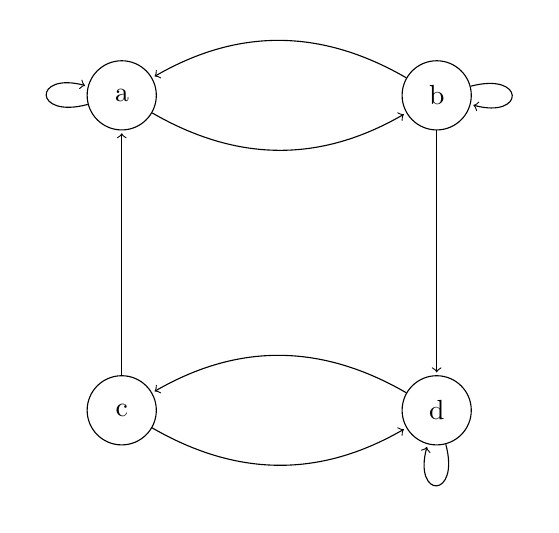
\begin{tikzpicture}[shorten >=1pt, node distance=4cm, on grid, auto]
    \node[state] (0) {a};
    \node[state] (1) [right=of 0] {b};
    \node[state] (2) [below=of 0] {c};
    \node[state] (3) [below=of 1] {d};
    \path[->]
     (0) edge [bend right]	node {} (1)
     (1) edge [bend right]  node {} (0)
     (2) edge               node {} (0)
     (3) edge [bend right]	node {} (2)
     (2) edge [bend right]  node {} (3)
     (1) edge				node {} (3)
     (0) edge [loop left]   node {} (0)
     (1) edge [loop right]  node {} (1)
     (3) edge [loop below]  node {} (3);
\end{tikzpicture}

\vfill


\end{enumerate} % end main problems

\end{document}

